\documentclass[11pt, letterpaper]{article}

\usepackage[margin=1in]{geometry}
\usepackage{amsmath, amssymb, amsthm}
\usepackage{tikz}
\usetikzlibrary{arrows.meta, patterns, decorations.pathmorphing, calc, decorations.markings}
\usepackage{hyperref}
\usepackage{fancyhdr}
\usepackage{titlesec}
\usepackage{enumitem}
\usepackage{xcolor}

% Colors
\definecolor{slabcolor}{RGB}{200, 180, 140}
\definecolor{slabdark}{RGB}{160, 140, 100}
\definecolor{accentblue}{RGB}{40, 80, 140}
\definecolor{arrowred}{RGB}{180, 50, 50}
\definecolor{arrowgreen}{RGB}{50, 140, 50}
\definecolor{seriestitle}{RGB}{80, 80, 80}
\definecolor{sheetcolor}{RGB}{220, 120, 60}
\definecolor{pillboxcolor}{RGB}{100, 160, 220}
\definecolor{fluxcolor}{RGB}{180, 50, 50}

% Headers
\pagestyle{fancy}
\fancyhf{}
\fancyhead[L]{\small\textcolor{seriestitle}{\textsc{Absurd Physics}}}
\fancyhead[R]{\small\textcolor{seriestitle}{Episode 1}}
\fancyfoot[C]{\thepage}
\renewcommand{\headrulewidth}{0.4pt}

% Section formatting
\titleformat{\section}{\Large\bfseries}{}{0em}{}[\vspace{2pt}\hrule\vspace{6pt}]
\titleformat{\subsection}{\large\bfseries}{}{0em}{}
\titleformat{\subsubsection}{\normalsize\bfseries\itshape}{}{0em}{}

% Custom environments
\newcommand{\seriesname}{\textsc{Absurd Physics}}

\begin{document}

% ================================================================
% TITLE PAGE
% ================================================================

\begin{center}
\vspace*{1.5cm}

{\fontsize{36}{42}\selectfont\bfseries\textcolor{accentblue}{ABSURD PHYSICS}}

\vspace{8pt}
{\large\textcolor{seriestitle}{\textit{A series exploring impossible worlds with both easy to understand proofs relying on symmetry that the non-mathematician can understand as well as proofs requiring complicated mathematics.}}}

\vspace{1.5cm}
\rule{0.6\textwidth}{0.5pt}
\vspace{1.5cm}

{\fontsize{24}{30}\selectfont Episode 1}

\vspace{10pt}

{\fontsize{28}{34}\selectfont\bfseries The Infinite Flat World}

\vspace{8pt}
{\large\textit{What would gravity be like on a planet shaped like\\an infinitely wide, uniform slab? It is possible to understand the answer with or without math. Without math, we can rely on a simple argument from symmetry.}}

\vspace{2cm}
\rule{0.6\textwidth}{0.5pt}
\end{center}

\vspace{1cm}

\subsection*{About This Series}

Welcome to \seriesname. This is the first installment of a series in which we take ridiculous, impossible scenarios---worlds that could never exist---and ask: \textit{what would the physics actually be like?}

Each article is split into two parts. \textbf{Part~1} builds intuition. No equations, no formalism---just careful reasoning about symmetry, geometry, and physical principles. If the argument is good enough, you should \textit{believe} the answer before seeing a single fancy math symbol.

\textbf{Part~2} is the mathematical proof. We roll up our sleeves, set up the math, and demonstrate rigorously that the intuitive answer is correct. If you're not a math person, Part~1 is designed to stand on its own and you can skip Part~2. If you \textit{are} a math person, Part~2 is where the real satisfaction lives.

Let's begin.

\newpage

% ================================================================
% NEWTONIAN GRAVITY
% ================================================================

\section*{A Quick Word About How Gravity Works}

Before we dive in, it's worth recalling how Newtonian gravity works, since everything in this article rests on it. The idea is simple: every piece of matter in the universe pulls on every other piece of matter. The force between two objects is proportional to the product of their masses and inversely proportional to the square of the distance between them. Double the distance, and the force drops to a quarter of what it was. Triple the distance, a ninth. This is Newton's law of universal gravitation, and for the kinds of scenarios we're considering---no black holes, no speeds near the speed of light, no absurdly strong gravitational fields---it's all we need.

The important consequence for us is this: when you're standing on a planet, the gravitational pull you feel is the \textit{combined} pull of every bit of matter in the planet, each chunk tugging on you according to that inverse-square law. On a sphere, things work out neatly---from the outside, a uniform sphere pulls as if all its mass were concentrated at its center. But there's nothing sacred about that result. It depends entirely on the spherical geometry. Change the shape, and the way all those individual pulls add up changes too, sometimes drastically. That's what makes this problem interesting.

% ================================================================
% THE SETUP
% ================================================================

\section*{The Setup}

Imagine a world that extends forever in every horizontal direction---an infinite flat slab of rock, uniform in thickness, uniform in density, stretching to the horizon and beyond it, forever. An endless horizontal pizza, if you will. No edges. No curvature. Just flat ground, above and below, going on without limit.

You're standing on top of it.

What does gravity feel like?

% ================================================================
% PART 1
% ================================================================

\section{The Argument from Symmetry}

We can figure out almost everything about gravity on the infinite pizza without doing any math at all. The only tool we need is \textbf{symmetry}---if a situation looks the same from two perspectives, the physics must be the same from each perspective.

\subsection{Gravity points straight down}

Stand anywhere on the surface of the slab. Define north, south, east, and west however you like. Look north. Look south. Look east. Look west. In every direction, the slab extends identically to infinity. There is nothing to distinguish one horizontal direction from another.

Now ask: does gravity pull me to the north?

It can't. There's nothing special about north. Every chunk of matter to your north, pulling you that way, is perfectly mirrored by an identical chunk to your south, pulling you back. The horizontal forces cancel---not approximately, but \textit{exactly}, by the perfect symmetry of the configuration.

The same argument kills every horizontal direction. Gravity can only point in the one direction that \textit{is} special: \textbf{straight down}, perpendicular to the slab. And this is true no matter where you stand, since every point on an infinite slab looks identical to every other point.

So without a single equation, we've nailed down the \textit{direction} of gravity everywhere. That's already a lot.

% ================================================================
% FIGURE: SYMMETRY ARGUMENT
% ================================================================

\begin{figure}[ht]
\centering
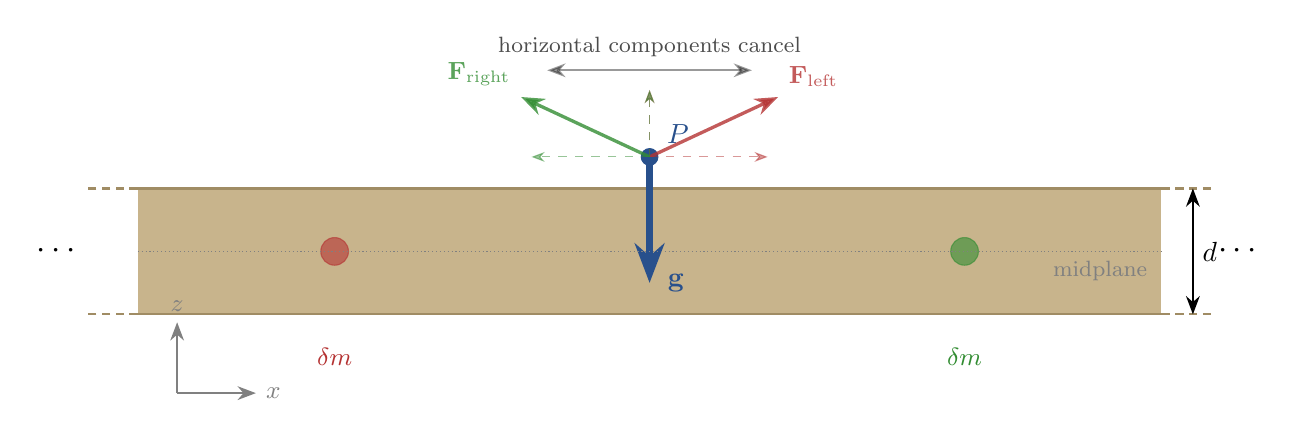
\begin{tikzpicture}[scale=1.0, >=Stealth]

  % --- Slab cross-section ---
  \fill[slabcolor] (-6.5, -0.8) rectangle (6.5, 0.8);
  \draw[thick, slabdark] (-6.5, 0.8) -- (6.5, 0.8);
  \draw[thick, slabdark] (-6.5, -0.8) -- (6.5, -0.8);

  % Dashed edges to suggest infinite extent
  \foreach \y in {-0.8, 0.8} {
    \draw[thick, densely dashed, slabdark] (-6.5, \y) -- (-7.2, \y);
    \draw[thick, densely dashed, slabdark] (6.5, \y) -- (7.2, \y);
  }

  \node at (-7.5, 0) {\large$\cdots$};
  \node at (7.5, 0) {\large$\cdots$};

  % Thickness label
  \draw[<->, thick] (6.9, -0.8) -- (6.9, 0.8);
  \node[right] at (6.9, 0) {$d$};

  % --- Observer point ---
  \filldraw[accentblue] (0, 1.2) circle (3pt);
  \node[above right, accentblue] at (0.1, 1.25) {$P$};

  % --- Symmetric mass elements and force arrows ---
  \filldraw[arrowred, opacity=0.6] (-4, 0) circle (5pt);
  \node[below, arrowred, font=\small] at (-4, -1.1) {$\delta m$};

  \filldraw[arrowgreen, opacity=0.6] (4, 0) circle (5pt);
  \node[below, arrowgreen, font=\small] at (4, -1.1) {$\delta m$};

  \draw[->, arrowred, very thick, opacity=0.8] (0, 1.2) -- ++(25:1.8)
    node[above right, font=\small] {$\mathbf{F}_{\text{left}}$};
  \draw[->, arrowred, dashed, opacity=0.5] (0, 1.2) -- ++(0:1.5);
  \draw[->, arrowred, dashed, opacity=0.5] (0, 1.2) -- ++(90:0.85);

  \draw[->, arrowgreen, very thick, opacity=0.8] (0, 1.2) -- ++(155:1.8)
    node[above left, font=\small] {$\mathbf{F}_{\text{right}}$};
  \draw[->, arrowgreen, dashed, opacity=0.5] (0, 1.2) -- ++(180:1.5);
  \draw[->, arrowgreen, dashed, opacity=0.5] (0, 1.2) -- ++(90:0.85);

  % Net force arrow (downward)
  \draw[->, accentblue, line width=2.5pt] (0, 1.2) -- ++(0, -1.6)
    node[right, font=\bfseries, xshift=2pt] {$\mathbf{g}$};

  \draw[<->, thick, opacity=0.4] (-1.3, 2.3) -- (1.3, 2.3);
  \node[above, font=\footnotesize, opacity=0.7] at (0, 2.35) {horizontal components cancel};

  \draw[densely dotted, gray] (-6.5, 0) -- (6.5, 0);
  \node[right, gray, font=\footnotesize] at (5.0, -0.25) {midplane};

  \draw[->, thick, gray] (-6.0, -1.8) -- (-5.0, -1.8) node[right, font=\small] {$x$};
  \draw[->, thick, gray] (-6.0, -1.8) -- (-6.0, -0.9) node[above, font=\small] {$z$};

\end{tikzpicture}
\caption{Cross-section of the infinite slab (thickness~$d$). For every mass element $\delta m$ to the left of point $P$, an identical element exists at the mirror position to the right. Their horizontal force components cancel exactly, leaving only the vertical pull.}
\label{fig:symmetry}
\end{figure}

\subsection{Gravity doesn't depend on where you stand}

Pick any two points on the surface, call them $A$ and $B$. What's different about them? Nothing. The slab is infinite, uniform, and featureless. An observer at $A$ and an observer at $B$ see \textit{exactly} the same arrangement of mass in every direction. So they must experience \textit{exactly} the same gravitational pull.

The gravitational field is the same everywhere on the surface. It's \textit{uniform}.

\subsection{The really strange part: gravity doesn't weaken with altitude}

This is the claim that raises eyebrows. When I first encountered it in an upper-level course on electromagnetic theory, it genuinely blew my mind. On Earth, fly higher and gravity weakens---you're moving away from the center of the planet. On the infinite pizza, fly upward and\ldots{} nothing changes. The pull is \textit{exactly the same} at any height above the surface.

Before getting to the symmetry argument, it helps to think about \textit{why} gravity weakens with altitude on a sphere in the first place. On a spherical planet, all the mass is concentrated in a finite region below you. Move away from it and every single chunk of that mass is now farther from you. Farther means weaker pull (inverse-square law), and since there's no new mass appearing to compensate, the total force drops.

On the infinite slab, the situation is fundamentally different. Move upward and yes, the patch of slab directly beneath your feet is now farther away, pulling more weakly. But here's what doesn't happen on a sphere: by moving upward, you've changed the \textit{angle} at which distant parts of the slab pull on you. When you're standing right on the surface, a chunk of slab a thousand kilometers away is pulling you almost perfectly \textit{horizontally}---it barely contributes to the downward force at all. It's almost parallel to you. But float a thousand kilometers up, and that same chunk is now well below you. Its pull has rotated from nearly horizontal to significantly downward. It's contributing much more to the force holding you down than it was before.

So as you rise, you lose pull from what's directly below you, but you \textit{gain} pull from the vast reaches of the slab stretching out to the sides---mass that was always there but wasn't contributing much when you were close to the surface. On a sphere, there's no ``vast reaches'' to pick up the slack. On an infinite slab, there's always more slab, extending forever, ready to compensate.

The symmetry argument makes this precise. Picture yourself floating a kilometer above the slab versus a million kilometers above it. In both cases, you look around and see an infinite flat plane below you, extending to infinity in all directions. There's no special length scale in this problem---no edge, no center, no radius. A view from one kilometer up looks just like a rescaled version of the view from a million kilometers up. There's nothing for the field to ``know'' about your altitude, and no mechanism for it to change.

\subsection{Inside the slab}

What if you tunnel into the pizza? Here, finally, something changes. As you descend, the mass above you starts pulling you \textit{up}, partially canceling the pull of the mass below. At the exact midplane---dead center of the slab---symmetry kicks in again, but now it's vertical symmetry. The mass above and below are mirror images. Every upward pull has a matching downward pull.

\textbf{Gravity is zero at the midplane.}

Between the surface and the midplane, the field drops smoothly from its surface value to zero. By a Gauss's Law argument (which we'll make precise in Part~2), the dropoff is \textit{linear}: halfway to the midplane, gravity is half its surface value. Simple as that.

\subsection{The complete picture}

Without writing a single equation, symmetry alone has told us:

\begin{itemize}[nosep]
  \item Gravity points straight down, everywhere, always.
  \item The field is the same at every point on the surface, and at every height above it.
  \item The field strength is \textit{constant} with altitude---it never weakens.
  \item Inside the slab, gravity decreases linearly to zero at the midplane.
  \item Below the midplane, everything mirrors: gravity reverses and pulls you back up toward the center.
\end{itemize}

\subsection{What if the slab had no thickness at all?}

Before we leave the symmetry arguments behind, it's worth asking: what if our infinite world were truly flat? Not a slab with some thickness, but an infinitely thin sheet---a mathematical plane with some mass per unit area but zero thickness.

The symmetry argument barely changes. The sheet is still infinite and uniform in all horizontal directions, so gravity still has to point straight down (or straight up, on the other side). And there's still no preferred location on the sheet, so the field is still uniform along the surface. The only thing we lose is the interior: there's no ``inside'' to tunnel into. You're either above the sheet or below it, and the midplane \textit{is} the sheet.

What about the constant-with-altitude property? The same reasoning applies, maybe even more cleanly. An infinite sheet looks the same from any height---there's no length scale at all now, not even a thickness to compare against. The field should be constant above and constant below.

There is one new wrinkle: the field has to be \textit{discontinuous} at the sheet. Above it, gravity pulls you down. Below it, gravity pulls you up. Right at the sheet, the two fields meet and there's a sudden jump. This makes physical sense---you're crossing an infinite plane of matter. We'll compute the size of the jump in Part~2, but symmetry already tells us the field above must equal the field below in magnitude (just opposite in direction), so the total jump is twice the one-sided value.

The zero-thickness case is actually \textit{simpler}---a cleaner version of the slab, with all the same qualitative features except the linear ramp through the interior, which collapses to a single discontinuous flip.

\subsection{Some consequences}

\textbf{No orbits.}\quad Orbital mechanics requires a force that weakens with distance. A satellite in a constant gravitational field doesn't orbit---it follows parabolic arcs, like a ball thrown in a room. Toss something sideways and it curves downward at the same rate no matter how fast it's going. Speed just makes the parabola wider.

\textbf{No escape.}\quad On a spherical planet, fly high enough and gravity fades away. You can reach escape velocity and leave forever. Here, the pull never lets up. No matter how fast you launch yourself upward, you'll eventually stop and fall back. Gravitational potential energy grows linearly with height, forever. You're trapped---not by some dramatic cosmic mechanism, but by the quiet, patient, unyielding constancy of the field.

\textbf{The atmosphere goes on forever.}\quad On Earth, the atmosphere thins exponentially with altitude partly because gravity weakens. Here, gravity \textit{doesn't} weaken, so the atmosphere still thins exponentially---but the scale height stays the same at every altitude. There's no sharp boundary. The air just gets thinner and thinner, never truly ending.

\subsection{Is it a black hole?}

Since there's no escape, you might wonder: is this just a black hole?

The ``no escape'' part does sound similar. In both cases, you're trapped---no amount of effort will get you to infinity. But that's where the resemblance ends. The experience of living on the infinite slab would be nothing like being near a black hole.

On the slab, nothing dramatic is happening. Gravity is gentle, constant, and frankly boring. You can jump, fly a jetpack, build a tower a trillion kilometers high---everything feels perfectly normal the whole time. You just can't \textit{stop} spending energy to stay up. Turn off the jetpack and you drift back down, always at the same acceleration, no matter how high you got. It's less like a cosmic trap and more like living in a room with a floor that extends forever. You're not being crushed or pulled apart. You're just\ldots{} in a room.

A black hole is a completely different beast. Inside the event horizon, it's not merely that you lack the energy to escape---the geometry of spacetime itself is warped so that \textit{all directions point inward}. Moving ``away'' from the singularity becomes as impossible as moving backward in time. No engine, no force, no amount of energy can even slow your infall. Space is funneling you in.

The best analogy for the infinite slab is actually the one you already know: standing in a room on Earth. You can't float away from the floor without spending energy, and when you stop jumping, you come back down. The infinite slab is that experience, extended forever in every direction. Above you, beside you, out to infinity. Cozy, not catastrophic.

So: trapped, yes. Black hole, not remotely. The friendliest prison in physics.

\newpage

% ================================================================
% PART 2
% ================================================================

\section{The Mathematical Proof}

Time to make all of this rigorous. We want to compute the gravitational field of an infinite uniform slab of thickness~$d$ and density~$\rho$, at an arbitrary point above (or inside) the slab. Then we'll handle the zero-thickness case as a special limit.

\textbf{A note on variables:} throughout this section, $d$ stands for the \textit{thickness} of the slab---\textbf{not} a differential and \textbf{not} time. We avoid using $t$ for thickness precisely because it's too easy to confuse with time.

The mathematical framework here is borrowed from electrostatics. Because Newtonian gravity and Coulomb's law share the same inverse-square structure, every technique for computing electric fields---superposition, Gauss's Law, the shell theorem---carries over directly to gravity with only minor sign changes.

\subsection{Setup}

Place the slab so that it occupies the region $-d/2 \leq z \leq d/2$, extending infinitely in the $x$ and $y$ directions. We want the gravitational acceleration $\mathbf{g}$ at an arbitrary point $P = (0, 0, z_0)$. By the symmetry arguments of Part~1, we already know $\mathbf{g}$ must point in the $-\hat{z}$ direction and depend only on~$z_0$. But let's prove it---and find the magnitude---by direct calculation.

\subsection{Method 1: Direct integration}

Consider a thin horizontal sheet of the slab at height~$z'$, with infinitesimal thickness~$dz'$. This sheet has surface mass density $\sigma = \rho \, dz'$. Our strategy: find the gravitational field of a single infinite sheet, then integrate over all sheets in the slab.

\subsubsection{Field of a single infinite sheet}

Take an infinite planar sheet of surface mass density~$\sigma$ lying in the $z = z'$ plane. We want the field at $P = (0, 0, z_0)$ with $z_0 > z'$.

% ================================================================
% FIGURE: RING INTEGRATION
% ================================================================

\begin{figure}[ht]
\centering
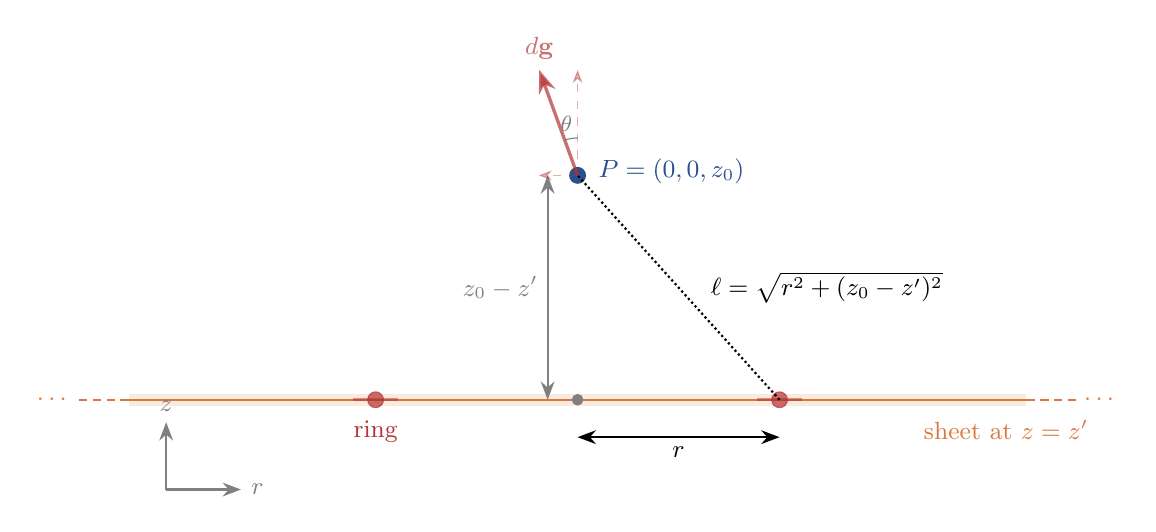
\begin{tikzpicture}[scale=0.95, >=Stealth]

  % --- The thin sheet ---
  \fill[sheetcolor, opacity=0.15] (-6, -0.08) rectangle (6, 0.08);
  \draw[sheetcolor, thick] (-6, 0) -- (6, 0);
  \draw[sheetcolor, thick, densely dashed] (-6, 0) -- (-6.7, 0);
  \draw[sheetcolor, thick, densely dashed] (6, 0) -- (6.7, 0);
  \node[sheetcolor, font=\small] at (-7.0, 0) {$\cdots$};
  \node[sheetcolor, font=\small] at (7.0, 0) {$\cdots$};

  % Sheet label
  \node[sheetcolor, font=\small, right] at (4.5, -0.4) {sheet at $z = z'$};

  % --- Ring element ---
  \draw[arrowred, very thick, opacity=0.5] (-3, 0) -- (-2.4, 0);
  \draw[arrowred, very thick, opacity=0.5] (2.4, 0) -- (3, 0);
  \filldraw[arrowred, opacity=0.7] (-2.7, 0) circle (3pt);
  \filldraw[arrowred, opacity=0.7] (2.7, 0) circle (3pt);
  \node[arrowred, font=\small, below] at (-2.7, -0.15) {ring};
  
  % --- r label ---
  \draw[<->, thick] (0, -0.5) -- (2.7, -0.5);
  \node[below, font=\small] at (1.35, -0.5) {$r$};

  % --- Field point P ---
  \filldraw[accentblue] (0, 3.0) circle (3pt);
  \node[accentblue, font=\small, right] at (0.15, 3.05) {$P = (0, 0, z_0)$};

  % --- Height label ---
  \draw[<->, thick, gray] (-0.4, 0) -- (-0.4, 3.0);
  \node[left, gray, font=\small] at (-0.4, 1.5) {$z_0 - z'$};

  % --- Distance ell ---
  \draw[densely dotted, thick] (2.7, 0) -- (0, 3.0);
  \node[right, font=\small] at (1.65, 1.5) {$\ell = \sqrt{r^2 + (z_0 - z')^2}$};

  % --- Force from right ring element ---
  \draw[->, arrowred, very thick, opacity=0.7] (0, 3.0) -- ++(110:1.5)
    node[above, font=\small] {$d\mathbf{g}$};

  % --- Decompose into vertical and horizontal ---
  \draw[->, arrowred, dashed, opacity=0.4] (0, 3.0) -- ++(180:0.52);
  \draw[->, arrowred, dashed, opacity=0.4] (0, 3.0) -- ++(90:1.41);
  
  % --- Angle theta ---
  \draw[gray] (0, 3.5) arc[start angle=90, end angle=110, radius=0.5];
  \node[gray, font=\footnotesize, above] at (-0.15, 3.45) {$\theta$};

  % --- Point directly below P ---
  \filldraw[gray] (0, 0) circle (2pt);

  % Coordinate axis
  \draw[->, thick, gray] (-5.5, -1.2) -- (-4.5, -1.2) node[right, font=\small] {$r$};
  \draw[->, thick, gray] (-5.5, -1.2) -- (-5.5, -0.3) node[above, font=\small] {$z$};

\end{tikzpicture}
\caption{Setting up the integral for a single infinite sheet. We decompose the sheet into concentric rings of radius~$r$ centered below the field point~$P$. Each ring exerts a gravitational pull along the line connecting it to~$P$, at distance~$\ell$. Only the vertical component (proportional to $\cos\theta$) survives after the horizontal parts cancel by symmetry.}
\label{fig:ring-integration}
\end{figure}

A ring of the sheet at radial distance~$r$ from the point directly below~$P$ has area $2\pi r \, dr$ and mass $dm = \sigma \cdot 2\pi r \, dr$. The distance from this ring to~$P$ is $\ell = \sqrt{r^2 + (z_0 - z')^2}$, and only the vertical component of the pull survives (the horizontal parts cancel by symmetry), giving a projection factor of $(z_0 - z')/\ell$. So the vertical field from this ring is:
\begin{equation}
  dg_z = -\frac{G \, \sigma \cdot 2\pi r \, dr}{\,r^2 + (z_0 - z')^2\,} \cdot \frac{z_0 - z'}{\sqrt{r^2 + (z_0 - z')^2}}.
\end{equation}

Integrate over $r$ from $0$ to $\infty$:
\begin{equation}
  g_z^{\,\text{sheet}} = -2\pi G \sigma \,(z_0 - z') \int_0^\infty \frac{r \, dr}{\bigl[\,r^2 + (z_0 - z')^2\,\bigr]^{3/2}}.
\end{equation}

Substitute $u = r^2 + (z_0 - z')^2$, so $du = 2r\,dr$:
\begin{align}
  g_z^{\,\text{sheet}} &= -2\pi G \sigma \,(z_0 - z') \cdot \frac{1}{2} \int_{(z_0 - z')^2}^{\infty} u^{-3/2}\,du \notag \\[6pt]
  &= -2\pi G \sigma \,(z_0 - z') \cdot \frac{1}{2} \left[-2\,u^{-1/2}\right]_{(z_0-z')^2}^{\,\infty} \notag \\[6pt]
  &= -2\pi G \sigma \,(z_0 - z') \cdot \frac{1}{|z_0 - z'|}.
\end{align}

For $z_0 > z'$, this gives:
\begin{equation}
  \boxed{\;g_z^{\,\text{sheet}} = -2\pi G \sigma\;}
  \label{eq:sheet}
\end{equation}

Stop and look at this. \textbf{The field of an infinite sheet doesn't depend on how far away you are.} Stand a meter from the sheet or a light-year from it---same pull. This is the key result, and everything else follows from it.

\subsubsection{Integrating over the slab}

The slab is just a stack of sheets from $z' = -d/2$ to $z' = d/2$, each with $\sigma = \rho \, dz'$. For a point above the slab ($z_0 > d/2$), every sheet pulls downward with the same strength:
\begin{equation}
  g_z = \int_{-d/2}^{\,d/2} \!\bigl(-2\pi G \rho\bigr)\,dz' = -2\pi G \rho \, d.
\end{equation}

So:
\begin{equation}
  \boxed{\;g = 2\pi G \rho\, d\;}
  \label{eq:slab}
\end{equation}

Constant. Independent of $z_0$. Exactly what we predicted.

\subsection{Method 2: Gauss's Law}

Gauss's Law for gravity states that for any closed surface~$S$:
\begin{equation}
  \oint_S \mathbf{g} \cdot d\mathbf{A} = -4\pi G\, M_{\text{enc}}
\end{equation}
where $M_{\text{enc}}$ is the total mass enclosed by~$S$. The sign difference from the electrostatic version reflects the fact that gravity is always attractive, while electric charges can repel.

\subsubsection{Above the slab}

Pick a ``Gaussian pillbox''---a short cylinder with its flat faces parallel to the slab, one face at height~$z_0$ above the slab and one at $-z_0$ below it (exploiting the up-down symmetry). Give the cylinder cross-sectional area~$A$.

% ================================================================
% FIGURE: GAUSSIAN PILLBOX
% ================================================================

\begin{figure}[ht]
\centering
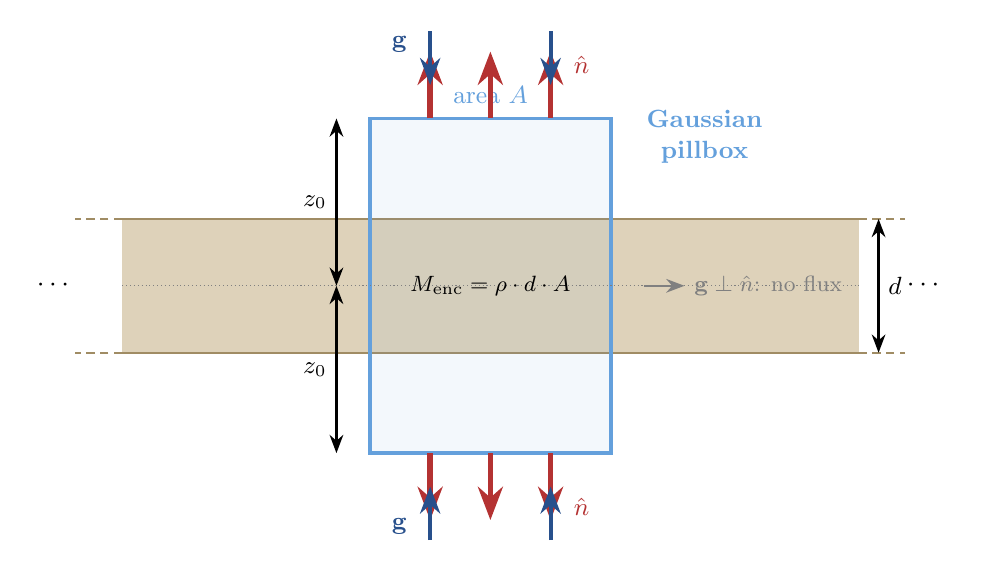
\begin{tikzpicture}[scale=0.85, >=Stealth]

  % --- Slab ---
  \fill[slabcolor, opacity=0.6] (-5.5, -1.0) rectangle (5.5, 1.0);
  \draw[thick, slabdark] (-5.5, 1.0) -- (5.5, 1.0);
  \draw[thick, slabdark] (-5.5, -1.0) -- (5.5, -1.0);

  \foreach \y in {-1.0, 1.0} {
    \draw[thick, densely dashed, slabdark] (-5.5, \y) -- (-6.2, \y);
    \draw[thick, densely dashed, slabdark] (5.5, \y) -- (6.2, \y);
  }
  \node at (-6.5, 0) {$\cdots$};
  \node at (6.5, 0) {$\cdots$};

  % --- Pillbox ---
  \draw[pillboxcolor, very thick, fill=pillboxcolor, fill opacity=0.08]
    (-1.8, -2.5) rectangle (1.8, 2.5);
  \draw[pillboxcolor, thick, densely dashed] (-1.8, -2.5) -- (-1.8, 2.5);
  \draw[pillboxcolor, thick, densely dashed] (1.8, -2.5) -- (1.8, 2.5);

  % Top face
  \draw[pillboxcolor, very thick] (-1.8, 2.5) -- (1.8, 2.5);
  % Bottom face
  \draw[pillboxcolor, very thick] (-1.8, -2.5) -- (1.8, -2.5);

  % Pillbox label
  \node[pillboxcolor, font=\small\bfseries] at (3.2, 2.5) {Gaussian};
  \node[pillboxcolor, font=\small\bfseries] at (3.2, 2.0) {pillbox};

  % Area label on top face
  \node[pillboxcolor, font=\small] at (0, 2.85) {area $A$};

  % --- Flux arrows on top face ---
  \draw[->, fluxcolor, line width=2pt] (-0.9, 2.5) -- (-0.9, 3.5);
  \draw[->, fluxcolor, line width=2pt] (0.0, 2.5) -- (0.0, 3.5);
  \draw[->, fluxcolor, line width=2pt] (0.9, 2.5) -- (0.9, 3.5);
  \node[fluxcolor, font=\small, right] at (1.1, 3.3) {$\hat{n}$};

  % --- g arrows pointing DOWN above slab ---
  \draw[->, accentblue, line width=1.5pt] (-0.9, 3.8) -- (-0.9, 3.0);
  \draw[->, accentblue, line width=1.5pt] (0.9, 3.8) -- (0.9, 3.0);
  \node[accentblue, font=\small, left] at (-1.1, 3.6) {$\mathbf{g}$};

  % --- Flux arrows on bottom face ---
  \draw[->, fluxcolor, line width=2pt] (-0.9, -2.5) -- (-0.9, -3.5);
  \draw[->, fluxcolor, line width=2pt] (0.0, -2.5) -- (0.0, -3.5);
  \draw[->, fluxcolor, line width=2pt] (0.9, -2.5) -- (0.9, -3.5);
  \node[fluxcolor, font=\small, right] at (1.1, -3.3) {$\hat{n}$};

  % --- g arrows pointing UP below slab ---
  \draw[->, accentblue, line width=1.5pt] (-0.9, -3.8) -- (-0.9, -3.0);
  \draw[->, accentblue, line width=1.5pt] (0.9, -3.8) -- (0.9, -3.0);
  \node[accentblue, font=\small, left] at (-1.1, -3.6) {$\mathbf{g}$};

  % --- No flux through sides annotation ---
  \draw[->, gray, thick] (2.3, 0) -- (2.9, 0);
  \node[gray, font=\footnotesize, right] at (2.9, 0) {$\mathbf{g} \perp \hat{n}$: no flux};

  % Height labels
  \draw[<->, thick] (-2.3, 0) -- (-2.3, 2.5);
  \node[left, font=\small] at (-2.3, 1.25) {$z_0$};
  \draw[<->, thick] (-2.3, -2.5) -- (-2.3, 0);
  \node[left, font=\small] at (-2.3, -1.25) {$z_0$};

  % Slab thickness
  \draw[<->, thick] (5.8, -1.0) -- (5.8, 1.0);
  \node[right, font=\small] at (5.8, 0) {$d$};

  % Midplane
  \draw[densely dotted, gray] (-5.5, 0) -- (5.5, 0);

  % Enclosed mass annotation
  \node[font=\footnotesize] at (0, 0) {$M_{\text{enc}} = \rho \cdot d \cdot A$};

\end{tikzpicture}
\caption{The Gaussian pillbox for the exterior field. The cylinder straddles the entire slab symmetrically. The gravitational field $\mathbf{g}$ points inward (toward the midplane) on both flat faces, and runs parallel to the curved sides, contributing no flux there. All the slab mass within the cylinder's cross-section is enclosed.}
\label{fig:pillbox}
\end{figure}

By symmetry, $\mathbf{g}$ points in $-\hat{z}$ above the slab and $+\hat{z}$ below it, with equal magnitude. On the curved sides, $\mathbf{g}$ is parallel to the surface (perpendicular to the outward normal), so no flux passes through the sides.

The flux through the top face is $-gA$ (field points inward, opposite to the outward normal). The bottom face also contributes $-gA$ (field points inward there too). So the total flux is:
\begin{equation}
  -2gA = -4\pi G\,(\rho \cdot d \cdot A).
\end{equation}

And we get:
\begin{equation}
  g = 2\pi G \rho\, d.
\end{equation}

Same answer. Three lines instead of a page of integration. That's the power of Gauss's Law when you've got enough symmetry to use it.

\subsubsection{Inside the slab}

Put the pillbox faces at $+z_0$ and $-z_0$, where $0 < z_0 < d/2$. Now the enclosed mass is just the portion of the slab between $-z_0$ and $+z_0$---thickness $2z_0$ instead of~$d$.
\begin{equation}
  -2g(z_0)\cdot A = -4\pi G\,(\rho \cdot 2z_0 \cdot A)
\end{equation}
\begin{equation}
  g(z_0) = 4\pi G \rho\, z_0
\end{equation}

Linear in~$z_0$, just as the symmetry argument predicted. At the midplane ($z_0 = 0$), gravity vanishes. At the surface ($z_0 = d/2$), we recover $g = 2\pi G \rho\,d$.

\subsection{Summary of the field profile}

\begin{equation}
  \boxed{\;g(z) = \begin{cases} 2\pi G \rho\, d & \text{for } |z| > d/2 \quad \text{(outside the slab)} \\[8pt] 4\pi G \rho\, |z| & \text{for } |z| \leq d/2 \quad \text{(inside the slab)} \end{cases}\;}
  \label{eq:profile}
\end{equation}

\noindent Direction: always toward the midplane.

% ================================================================
% FIGURE: FIELD PROFILE
% ================================================================

\begin{figure}[ht]
\centering
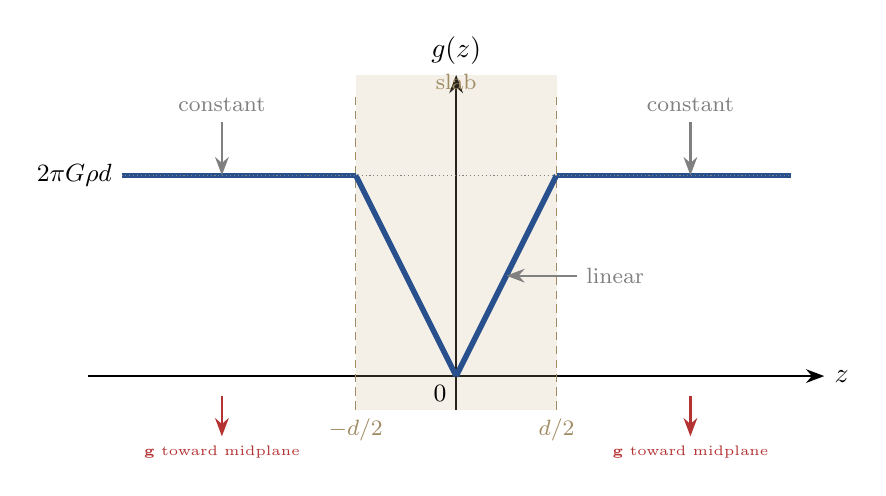
\begin{tikzpicture}[scale=0.85, >=Stealth]

  % Axes
  \draw[->, thick] (-5.5, 0) -- (5.5, 0) node[right] {$z$};
  \draw[->, thick] (0, -0.5) -- (0, 4.5) node[above] {$g(z)$};

  % Slab region shading
  \fill[slabcolor, opacity=0.2] (-1.5, -0.5) rectangle (1.5, 4.5);
  \draw[slabdark, densely dashed] (-1.5, -0.5) -- (-1.5, 4.2);
  \draw[slabdark, densely dashed] (1.5, -0.5) -- (1.5, 4.2);

  % Slab labels
  \node[slabdark, font=\footnotesize] at (-1.5, -0.8) {$-d/2$};
  \node[slabdark, font=\footnotesize] at (1.5, -0.8) {$d/2$};
  \node[slabdark, font=\footnotesize] at (0, 4.4) {slab};

  % The field profile
  % Left exterior: constant
  \draw[accentblue, line width=2pt] (-5.0, 3.0) -- (-1.5, 3.0);

  % Interior: linear ramp
  \draw[accentblue, line width=2pt] (-1.5, 3.0) -- (0, 0);
  \draw[accentblue, line width=2pt] (0, 0) -- (1.5, 3.0);

  % Right exterior: constant
  \draw[accentblue, line width=2pt] (1.5, 3.0) -- (5.0, 3.0);

  % Dashed level line for g_surface
  \draw[gray, densely dotted] (-5.0, 3.0) -- (5.0, 3.0);
  \node[left, font=\small] at (-5.0, 3.0) {$2\pi G\rho d$};

  % Annotations
  \draw[<-, thick, gray] (-3.5, 3.0) -- (-3.5, 3.8);
  \node[above, gray, font=\footnotesize] at (-3.5, 3.8) {constant};

  \draw[<-, thick, gray] (3.5, 3.0) -- (3.5, 3.8);
  \node[above, gray, font=\footnotesize] at (3.5, 3.8) {constant};

  \draw[<-, thick, gray] (0.75, 1.5) -- (1.8, 1.5);
  \node[right, gray, font=\footnotesize] at (1.8, 1.5) {linear};

  % Zero label
  \node[below left, font=\small] at (0, 0) {$0$};

  % Direction arrows
  \draw[->, arrowred, thick] (-3.5, -0.3) -- (-3.5, -0.9);
  \node[arrowred, font=\tiny, below] at (-3.5, -0.9) {$\mathbf{g}$ toward midplane};
  \draw[->, arrowred, thick] (3.5, -0.3) -- (3.5, -0.9);
  \node[arrowred, font=\tiny, below] at (3.5, -0.9) {$\mathbf{g}$ toward midplane};

\end{tikzpicture}
\caption{The gravitational field magnitude $g(z)$ as a function of position. Outside the slab, the field is constant at $2\pi G\rho d$. Inside, it drops linearly to zero at the midplane. The direction is always toward the midplane: downward above, upward below.}
\label{fig:field-profile}
\end{figure}

\subsection{The zero-thickness limit}

Now let's take the thickness to zero. Shrink $d \to 0$ while keeping the total surface mass density $\sigma = \rho\, d$ fixed. (If we let $\sigma$ vanish too, the field just disappears---not very interesting.)

The exterior field becomes:
\begin{equation}
  g = 2\pi G \sigma
\end{equation}

This is exactly equation~(\ref{eq:sheet})---no surprise, since a slab of zero thickness \textit{is} a sheet. The field is constant above and constant below, with magnitude $2\pi G\sigma$ on each side.

What about the interior? There isn't one anymore. The linear ramp from $g = 2\pi G \rho\, d$ at the surface down to $g = 0$ at the midplane has been crushed to a single point. The field jumps discontinuously from $+2\pi G \sigma$ (pointing down, just above) to $-2\pi G \sigma$ (pointing up, just below)---a total discontinuity of $4\pi G \sigma$.

% ================================================================
% FIGURE: ZERO-THICKNESS FIELD
% ================================================================

\begin{figure}[ht]
\centering
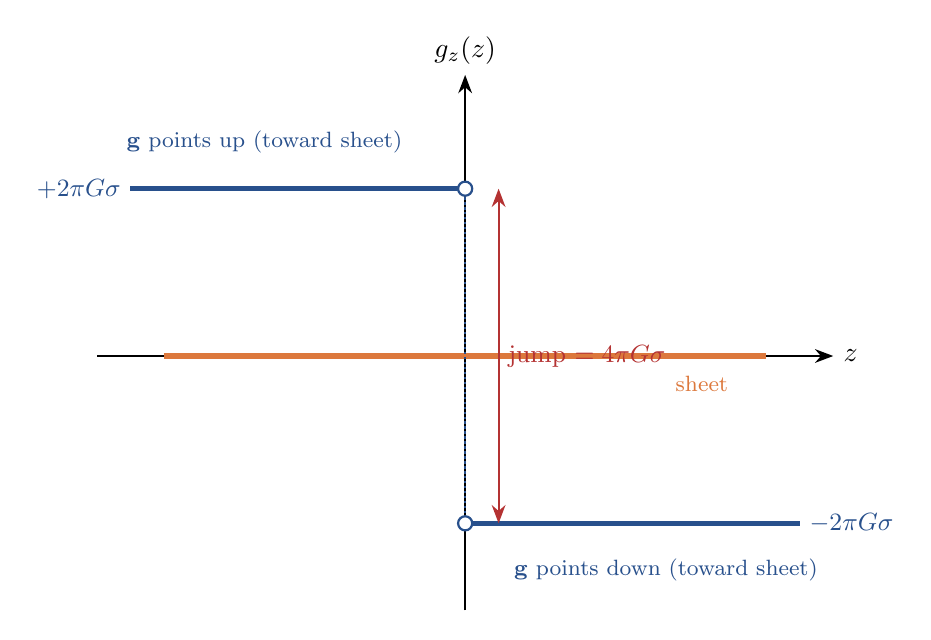
\begin{tikzpicture}[scale=0.85, >=Stealth]

  % Axes
  \draw[->, thick] (-5.5, 0) -- (5.5, 0) node[right] {$z$};
  \draw[->, thick] (0, -3.8) -- (0, 4.2) node[above] {$g_z(z)$};

  % The sheet
  \draw[sheetcolor, line width=2pt] (-4.5, 0) -- (4.5, 0);
  \node[sheetcolor, font=\footnotesize, below right] at (3.0, -0.15) {sheet};

  % Field above: constant negative (pointing down = toward sheet)
  \draw[accentblue, line width=2pt] (0.08, -2.5) -- (5.0, -2.5);
  \node[accentblue, font=\small, right] at (5.0, -2.5) {$-2\pi G\sigma$};

  % Field below: constant positive (pointing up = toward sheet)
  \draw[accentblue, line width=2pt] (-5.0, 2.5) -- (-0.08, 2.5);
  \node[accentblue, font=\small, left] at (-5.0, 2.5) {$+2\pi G\sigma$};

  % Discontinuity
  \draw[accentblue, densely dotted, thick] (0, -2.5) -- (0, 2.5);
  \filldraw[white] (0, 2.5) circle (3pt);
  \draw[accentblue, thick] (0, 2.5) circle (3pt);
  \filldraw[white] (0, -2.5) circle (3pt);
  \draw[accentblue, thick] (0, -2.5) circle (3pt);

  % Jump annotation
  \draw[<->, thick, arrowred] (0.5, -2.5) -- (0.5, 2.5);
  \node[arrowred, font=\small, right] at (0.5, 0) {jump $= 4\pi G\sigma$};

  % Direction annotations
  \node[accentblue, font=\footnotesize] at (3.0, -3.2) {$\mathbf{g}$ points down (toward sheet)};
  \node[accentblue, font=\footnotesize] at (-3.0, 3.2) {$\mathbf{g}$ points up (toward sheet)};

\end{tikzpicture}
\caption{The $z$-component of the gravitational field for a zero-thickness infinite sheet. The field is constant on each side but flips sign at the sheet, producing a discontinuity of magnitude $4\pi G\sigma$. This is the $d \to 0$ limit of the slab profile in Figure~\ref{fig:field-profile}---the linear ramp has collapsed to a single jump.}
\label{fig:sheet-profile}
\end{figure}

We can also get this straight from Gauss's Law. Put a pillbox straddling the sheet, one face just above, one just below. The enclosed mass is $\sigma A$, and the two faces each see a field of magnitude~$g$ pointing inward:
\begin{equation}
  -2gA = -4\pi G\,\sigma A \quad\implies\quad g = 2\pi G\sigma.
\end{equation}

Same answer. The zero-thickness case isn't really a different problem---it's the same problem with the interior removed. Every qualitative feature (constant field, no orbits, no escape) carries over unchanged. The only thing that disappears is the smooth linear transition through the middle, replaced by an instantaneous flip.

\subsection{A numerical example}

Suppose our pizza has Earth-like density ($\rho = 5{,}500\;\text{kg/m}^3$) and is 100~km thick. Then:
\begin{equation}
  g = 2\pi \,(6.674 \times 10^{-11})(5{,}500)(100{,}000) \approx 0.23\;\text{m/s}^2.
\end{equation}

That's about 2.3\% of Earth's surface gravity. You'd feel like you weigh about five pounds---gentle, but noticeable. And since gravity scales linearly with thickness, a slab about 4{,}300~km thick with the same density would give you Earth-standard $9.8\;\text{m/s}^2$.

\subsection{No escape velocity}

The gravitational potential above the slab is:
\begin{equation}
  \Phi(z) = -2\pi G \rho\, d \cdot z + \text{const.}
\end{equation}

This grows without bound as $z \to \infty$. To escape to infinity, you'd need infinite kinetic energy. There is no escape velocity. You're stuck, period.

This holds for the zero-thickness sheet too. Replace $\rho\,d$ with $\sigma$ and the potential is $\Phi(z) = -2\pi G\sigma\, z + \text{const.}$---still unbounded, still no escape.

% ================================================================
% CLOSING
% ================================================================

\section*{Closing Thoughts}

The infinite pizza is one of the cleanest results in gravitational physics---a case where real geometry falls away and you're left with a perfectly uniform, perfectly constant gravitational field. The math is accessible to anyone who's taken first-year physics, and the result is weird enough to give even experienced physicists a moment of pause.

More than anything, it's a reminder that our intuitions about gravity---it weakens with distance, there's always an escape velocity, orbits are possible---are really just intuitions about \textit{spheres}. We live on one, so we've internalized its rules. Change the geometry, and the rules change completely.

\vspace{1cm}
\begin{center}
\rule{0.4\textwidth}{0.5pt}\\[8pt]
{\small\textit{Next time on \seriesname: we'll explore what happens when you do something even stranger.}}\\[4pt]
{\footnotesize \seriesname{} is a series about impossible worlds and real mathematics.}
\end{center}

\vspace{1cm}

\subsection*{Further Reading}

The mathematics in Part~2 is adapted from Chapter~2 of David~J.\ Griffiths' \textit{Introduction to Electrodynamics} (4th edition, Cambridge University Press, 2017). Although the book is about electrostatics, not gravity, the two theories share the same inverse-square force law, so every calculation carries over with only minor sign changes. If you want to see these techniques developed properly and at length, Chapter~2 of Griffiths is the place to go---it's one of the best-written textbook chapters in all of physics.

\end{document}
